\documentclass[a4paper,12pt]{article}
\usepackage{amsmath}
\usepackage[margin=2cm]{geometry}
\usepackage{graphicx}
\usepackage{bbding}
\usepackage[usenames,dvipsnames]{color}
\usepackage{multirow}
\usepackage[table]{xcolor}  
\usepackage{footnote} 
\usepackage[bottom]{footmisc}     
\usepackage{titletoc}
\usepackage{url}

\usepackage[bookmarksnumbered,breaklinks]{hyperref}
\usepackage{breakurl}
\def\UrlBreaks{\do\/\do-}
\usepackage{tabularx}
\usepackage{bookmark}
\usepackage{siunitx}
\usepackage{hhline}
\usepackage{booktabs}
\usepackage{caption}
\usepackage{subcaption}
\usepackage{fixltx2e}
\usepackage{amssymb}
\usepackage[T1]{fontenc}
\usepackage{textcomp}
\newcommand{\angstrom}{\textup{\AA}}
\def \be {\begin{equation}}
\def \ee {\end{equation}}
\usepackage{listings}
\usepackage{braket}
\usepackage[nottoc, notlof, notlot]{tocbibind}
\newcommand{\setflag}{\newif \ifwhole \wholetrue}
\setflag 
\usepackage{appendix}
\renewcommand\tiny{\@setfontsize\small{10}{11}}

\begin{document}
\title{\textbf{\Huge { 2D Schroedinger-Poisson Solver: Documentation}}}
\date{\today}
%\author{Augustin Bussy} 
\maketitle

\section{Introduction}

This code aims at self-consistently solving the coupled Schroedinger-Poisson equations in 2D materials. More accurately, it is designed to simulate nanosheets of a single material with regions of different strains. The Schroedinger equation is in 1D, meaning that the strain can vary on a single axis ($x$), as illustrated in figure \ref{fig:example1}. Moreover, the material is assumed to be infinite in the $y$-direction and periodic in the $x$-direction.\\

Two types of calculations can be made: single-point or map. The former precisely simulates a specific setup described in an input file to produce a band or a carrier density profile. This is a useful tool for experiments as it allows to simulated any strain profile (almost continuously). The map calculation screens over different setups of strained/unstrained material to investigate insulator to conductor phase transitions.\\

This code uses a multi-scale approach, meaning that the materials properties must come from DFT calculations. The user has to provide vital quantities such as effective masses and polarization charges  for different strains. The properties for at least 4-5 strains should be provided for accurate fitting. It is also not recommended to extrapolate strains larger than those coming from DFT, as the trends could change.

\begin{figure} [h]
\begin{center}
\captionsetup{width=0.8\textwidth}
\centerline{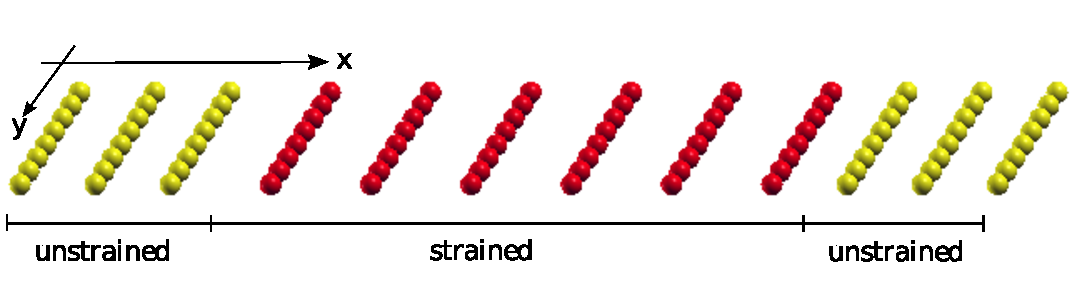
\includegraphics[width=12cm,angle=0]{img/example1}}
\caption{Example of simulation setup: Periodic alternation of strained and unstrained material}
\label{fig:example1} 
\end{center}
\end{figure}


\section{Setting up the code}
The code itself is contained in 4 files: \texttt{2Dschrpoisson.py}, \texttt{schrpoisson\_wire2.f90}, \texttt{schrpoisson\_wire2.pyf} and \texttt{Makefile}. The bulk of the numerical part being written in FORTRAN, one must compile using the \texttt{make} command. The code is now ready to run using the following command in the code folder:\\

\texttt{python 2Dschrpoisson.py \{material\_properties\}.json  \{calculation\_input\}.json}\\

\noindent Note that the Python path to the input json files must be provided.

\section{Input}
Two input files are necessary to every calculation: one containing the materials properties and the other the calculation setup. All input files must be stored in the input folder.
\subsection{Materials Properties File}
The file containing the properties of the material at different strains must be in the \texttt{json} format, in the form of a python dictionary. The following example is taken from the SnSe\_example.json in the input folder. Note that the properties of the unstrained material are \textbf{mandatory} and must be given under the "0.00" key.\\

\begin{tabbing}
\{"0.00": \{ \= "alpha\_xx": 10.22,\\
	\> "x\_lat": 4.408,\\
	\> "y\_lat": 4.288,\\
	\> "polarization\_charge": 0.0,\\
	\> "vacuum\_level": 3.471695,\\
	\> "valence\_gamma": \{ \="energy": -1.508255819,\\
			     \>\>"conf\_mass": 1.755925079,\\
			     \>\>"DOS\_mass": 2.7330924,\\
			     \>\>"degeneracy": 1\\
			     \>\>\},\\
	   \>"valence\_gamma-X": \{\="energy": -0.8832657543,\\
			      \>\> "conf\_mass": 0.125168454,\\
			      \> \>"DOS\_mass": 0.159070572,\\
			       \>\>"degeneracy": 2\\
			      \>\> \},\\
	   \>"valence\_gamma-Y": \{\="energy": -1.064317364,\\
			      \>\> "conf\_mass": 0.109554071,\\
			      \>\> "DOS\_mass": 0.159511425,\\
			      \>\> "degeneracy": 2\\
			      \>\>\},\\
	   \>"conduction\_gamma": \{\="energy": 0.6090962485,\\
				\>\>"conf\_mass": 2.741100107,\\
				\>\>"DOS\_mass": 2.994158008,\\
			        \>\>"degeneracy": 1\\
			       \>\>\},\\
	  \> "conduction\_gamma-X": \{\="energy": 0.0902128713,\\
				\>\>  "conf\_mass": 0.110807373,\\
				\>\>  "DOS\_mass": 0.190387132,\\
			        \>\>  "degeneracy": 2\\
				\>\> \},\\
	   \>"conduction\_gamma-Y": \{\="energy": 0.05720314215,\\
				\>\>  "conf\_mass": 0.131542031,\\
				  \>\>"DOS\_mass": 0.130378261,\\
			          \>\>"degeneracy": 2\\
				 \>\>\}\\
	 \>\},\\
\ "0.01": \{\=...\\
	  \>\},\\
...\}\\
\end{tabbing}

\begin{itemize}
\item The "0.00" key: the first key is the strain of a the material and the assigned value is a subdictionary with all the relevant peoperties. The "0.00" key is mendatory.

\item The "alpha\_xx" key: this refers to the polarizability of the strained material in \angstrom. $x$ is the direction along which different strains/materials alternate

\item The "x\_lat" and "y\_lat" keys: the lattice parameters of the unit cell in \angstrom. Only needed for the unstrained material

\item The "polarization\_charge" key: the polarization charge at the edge of the material in units of electron per unit cell width, \textit{i.e.} e/b.

\item The "vacuum\_level" key: Self-explanatory, needed to align energy levels across the setup (in eV).

\item The energy levels keys: They need to either contain the word \texttt{valence} or \texttt{conduction}, which is needed by the code. The assigned value is a subdictionary with the energy of the band extremum (eV), the confinement and density of states (DOS) masses (respectively effective masses in $x$ and $y$ direction) and the degeneracy of the energy level in the first BZ.

\end{itemize}

\subsection{Calculation Input File}
Each type of calculation , single-point or map, has its own input file template. However, both of them are required to be \texttt{json} files in the form of a python dictionary. The following examples can be found in the input folder and can be generated using the \texttt{create\_calc\_input.py} script.

\subsubsection{Single-Point Calculation}

\begin{tabbing}
\{ \ \= \\
          \>"calculation": "single\_point", \\
           \>"out\_dir": "single\_point\_output", \\
           \>"smearing": true, \\
           \>"KbT": 0.005,\\
           \>"max\_iteration": 1000, \\
          \>"plot\_fit": false, \\
         \> "nb\_of\_states\_per\_band": 2, \\
          \>"delta\_x": 0.5, \\
          \>"setup": \{ \= \\
                   \>\> "slab1": \{ \= \\
                             \>\>\> "polarization": "positive", \\
                               \>\>\>"strain": 0.0, \\
                               \>\>\>"width": 15.0\\
                    \>\>\}, \\
                    \>\>"slab2": \{\= \\
                               \>\>\>"polarization": "positive",\\ 
                               \>\>\>"strain": 0.08, \\
                               \>\>\>"width": 30.0\\
                    \>\>\},\\
                    \>\>"slab3": \{\= \\
                               \>\>\>"polarization": "positive",\\ 
                              \>\>\> "strain": 0.0, \\
                               \>\>\>"width": 15.0\\
                    \>\>\}, \\

          \>\}, \\


\}\\
\end{tabbing}

\begin{itemize}
\item The "calculation" key: the value \texttt{"single\_point"} indicates the type of calculation

\item The "out\_dir" key: indicates the name of the folder where the output data is dumped

\item The "smearing" key: If \texttt{true}, a Marzari-Vanderbilt smearing is imposed for the electron distribution. It helps for the convergence of the self-consistent Schroedinger-Poisson loop and allows better comparisons with DFT calculations.

\item The "KbT" key: In case of smearing, this is the imposed electronic temperature (Ry)

\item The "max\_iteration" key: The number of allowed steps for the self-consistent Schroedinger-Poisson loop, 1000 is a safe number.

\item The "plot\_fit" key: If \texttt{true}, the fitting of materials properties for any strain is displayed in a series of graphs

\item The "nb\_of\_states\_per\_band" key: To limit the size of the output data. Here, only two quantum states per band (6 in total) will be reported

\item The "delta\_x" key: The size of the discretization step in space (\angstrom)

\item The "setup" key: The assigned value is a subdictionary with the description of each slab forming the general setup. For each layer, one has to specify the "polarization" (positive or negative, positive if holes accumulate towards larger $x$), the "strain" of the material and the "width" of the slab (\angstrom). There is no limit to the numbers of layers but the keys must follow the logic, \textit{i.e.} "slab+integer". It is not recommended to include strains higher than the largest one in the material properties file. It is also \textbf{mandatory} that the first and the last slabs have identical strain, since the code does not cope with polarization charges at the edges of the cell.
\end{itemize}

\subsubsection{Map Calculation}

\begin{tabbing}
\{\= \\
	 \> "calculation": "map", \\
	 \>"out\_dir": "map\_output", \\
          \>"smearing": true, \\
           \>"KbT": 0.005, \\
           \>"max\_iteration": 1000, \\
           \>"plot\_fit": false, \\
          \>"nb\_of\_steps": 200, \\
	 \> "upper\_delta\_x\_limit": 0.5, \\
         \> "strain": \{ \= \\
                    \>\>"max\_strain": 0.1, \\
                    \>\>"min\_strain": 0.0, \\
                    \>\>"strain\_step": 0.01\\
         \> \}, \\
          \>"width": \{ \= \\
                    \>\>"min\_width": 10.0,\\ 
                    \>\>"width\_step": 5.0, \\
                    \>\>"max\_width": 60.0\\
          \>\}, \\

\}\\
\end{tabbing}


\begin{itemize}
\item The "calculation" key: the value \texttt{"map"} indicates the type of calculation

\item The "out\_dir" key: indicates the name of the folder where the output data is dumped

\item The "smearing" key: If \texttt{true}, a Marzari-Vanderbilt smearing is imposed for the electron distribution. It helps for the convergence of the self-consistent Schroedinger-Poisson loop and allows better comparisons with DFT calculations.

\item The "KbT" key: In case of smearing, this is the imposed electronic temperature (Ry)

\item The "max\_iteration" key: The number of allowed steps for the self-consistent Schroedinger-Poisson loop, 1000 is a safe number.

\item The "plot\_fit" key: If \texttt{true}, the fitting of materials properties for any strain is displayed in a series of graphs

\item The "nb\_of\_steps" key: Since a wide range of setup sizes is spanned in a map calculation, a common step size might be a problem. It is instead dynamically adapted as $\Delta x = \frac{L_{tot}}{\text{nb\_of\_steps}}$

\item The "upper\_delta\_x\_limit" key: In case a limit should be imposed on the step size: $\Delta x = min(\frac{L_{tot}}{nb\_of
\_steps}, \text{upper\_delta\_x\_limit})$

\item The "strain" key: The assigned value is a subdictionary with the lower and upper bound ("min\_strain" and "max\_strain") of the strains over which calculations will be done. 

\item The "width" key: The assigned value is a subdictionary with the lower and upper bound ("min\_width" and "max\_width") of the width over which calculations will be done. The width refers to the unstrained material, the size of the strained slab is computed via $L_{strained} = (1+\epsilon)L_{unstrained}$. In this example, 121 single-point calculations will be conducted with every combination of strain $\epsilon = 0.0, 0.01,...,0.1$ and width $L = 10.0, 15.0,..., 60.0$.


\end{itemize}





\section{Output}

\subsection{Single-Point Calculation}
In single-point calculations, 3 output files are generated. The first  one (\texttt{general\_info.txt}) contains general information such as the number of iterations needed, convergence parameters or total free carrier density. The second one, \texttt{band\_data.txt}, contains all the necessary information to produce a band profile (Fermi energy, potential profile of each band, their respective quantum states, etc.) Finally, the last file (\texttt{density\_profile.txt}) contains the free electrons and holes density as a function of position, in different units.



\subsection{Map Calculation}
Map calculations produce a single output file in which, among others, the total electron density is given for each strain/width combination in order to produce a map.

\end{document}